\documentclass[aspectratio=169]{beamer}

\usepackage[utf8]{inputenc}
\usepackage{graphicx}
\usepackage{tikz}
\usetikzlibrary{positioning, arrows.meta, calc}
\usepackage{pifont}
\usepackage{fontawesome5}

\usefonttheme{professionalfonts}

\usetheme{Madrid}
\definecolor{slideblue}{RGB}{100, 160, 210}
\definecolor{statred}{RGB}{180, 50, 50}
\definecolor{ucdgreen}{RGB}{0, 102, 51}
\usecolortheme[named=slideblue]{structure}
\setbeamertemplate{navigation symbols}{}
\setbeamersize{text margin left=7mm, text margin right=7mm}
\setbeamertemplate{headline}{}
\setbeamercolor{upper separation line foot}{bg=white}
\setbeamercolor{middle separation line foot}{bg=white}
\setbeamercolor{lower separation line foot}{bg=white}
\setbeamercolor{author in head/foot}{fg=slideblue!70!black, bg=slideblue!15}
\setbeamercolor{title in head/foot}{fg=slideblue!70!black, bg=slideblue!15}
\setbeamercolor{date in head/foot}{fg=slideblue!70!black, bg=slideblue!15}
\setbeamertemplate{footline}{%
  \leavevmode%
  \hbox{%
    \begin{beamercolorbox}[wd=.333333\paperwidth,ht=2.25ex,dp=1.5ex,center]{author in head/foot}%
      \usebeamerfont{author in head/foot}\insertshortauthor
    \end{beamercolorbox}%
    \begin{beamercolorbox}[wd=.333333\paperwidth,ht=2.25ex,dp=1.5ex,center]{title in head/foot}%
      \usebeamerfont{title in head/foot}\insertshorttitle
    \end{beamercolorbox}%
    \begin{beamercolorbox}[wd=.333333\paperwidth,ht=2.25ex,dp=1.5ex,right]{date in head/foot}%
      \usebeamerfont{date in head/foot}%
      \insertframenumber{} / \inserttotalframenumber\hspace*{2ex}
    \end{beamercolorbox}}%
  \vskip2pt%
}

\title[ANTICIPATE WG1/WG2 Workshop]{}
\author[Lainey Ward]{}
\institute[]{}
\date{}

\begin{document}

% --------------------------------------------------
% SLIDE 1: Title
% --------------------------------------------------
\begin{frame}

    \vspace{1.8cm}
    \begin{center}
        {\LARGE\bfseries\color{slideblue!90!black}
         Evaluation of ECMWF S2S Forecasts\\[0.3em]
         over Ireland for Multi-Hazard Applications}

        \vspace{1.2em}
        {\large Lainey Ward}

        \vspace{0.5em}
        {\footnotesize Decarb-AI Centre, University College Dublin}
    \end{center}

    \vspace{0.8em}
    \begin{center}
        
\includegraphics[height=0.85cm, trim=0 0 0 5, clip]{ucd.png}%
        \hspace{2em}%
        
\includegraphics[height=0.85cm]{InnovateforIreland.png}%
        \hspace{2em}%
        
\includegraphics[height=0.85cm]{AIBBANK.png}
    \end{center}

\end{frame}

% --------------------------------------------------
% SLIDE 2: What happens when drought becomes flood?
% --------------------------------------------------
\begin{frame}{What Happens When Drought Becomes Flood?}

    \begin{columns}[c, totalwidth=\textwidth]

        \begin{column}{0.55\textwidth}
            \centering
            \vspace{1.5em}
            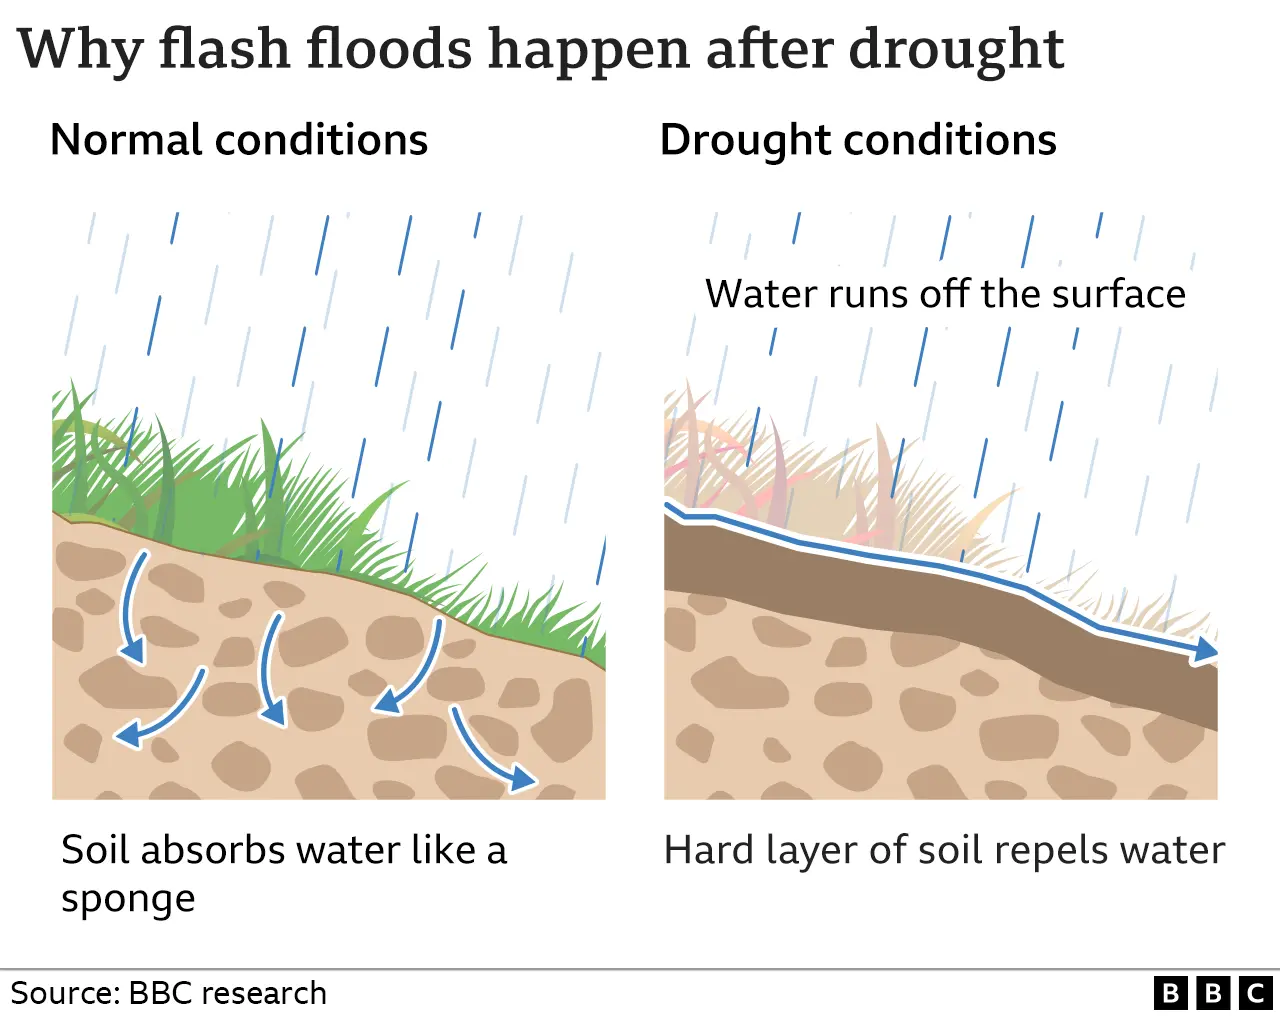
\includegraphics[width=\textwidth, keepaspectratio,
                trim=0 80 0 100, clip]
                {Soil.png}\\[0.2em]
            {\tiny\color{gray!65} Adapted from BBC Research (2022)}
        \end{column}

        \begin{column}{0.43\textwidth}
            \centering
            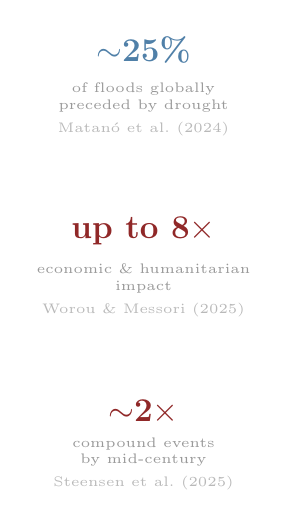
\begin{tikzpicture}

                \node[font=\large\bfseries, text=slideblue!80!black]
                    at (0, 2.5) {{$\sim$}25\%};
                \node[font=\tiny, text=gray!80, align=center]
                    at (0, 1.9) {of floods globally\\preceded by drought};
                \node[font=\tiny, text=gray!55]
                    at (0, 1.5) {Matan\'o et al.\ (2024)};

                \node[font=\large\bfseries, text=statred!80!black]
                    at (0, 0.2) {up to 8{$\times$}};
                \node[font=\tiny, text=gray!80, align=center]
                    at (0, -0.4) {economic \& humanitarian\\impact};
                \node[font=\tiny, text=gray!55]
                    at (0, -0.8) {Worou \& Messori (2025)};

                \node[font=\large\bfseries, text=statred!80!black]
                    at (0, -2.1) {{$\sim$}2{$\times$}};
                \node[font=\tiny, text=gray!80, align=center]
                    at (0, -2.6) {compound events\\by mid-century};
                \node[font=\tiny, text=gray!55]
                    at (0, -3.0) {Steensen et al.\ (2025)};

            \end{tikzpicture}
        \end{column}

    \end{columns}

\end{frame}

% --------------------------------------------------
% SLIDE 3: Has anyone tried to forecast this?
% --------------------------------------------------
\begin{frame}{Has Anyone Tried to Forecast This?}

    \centering
    \vspace{0.5em}
    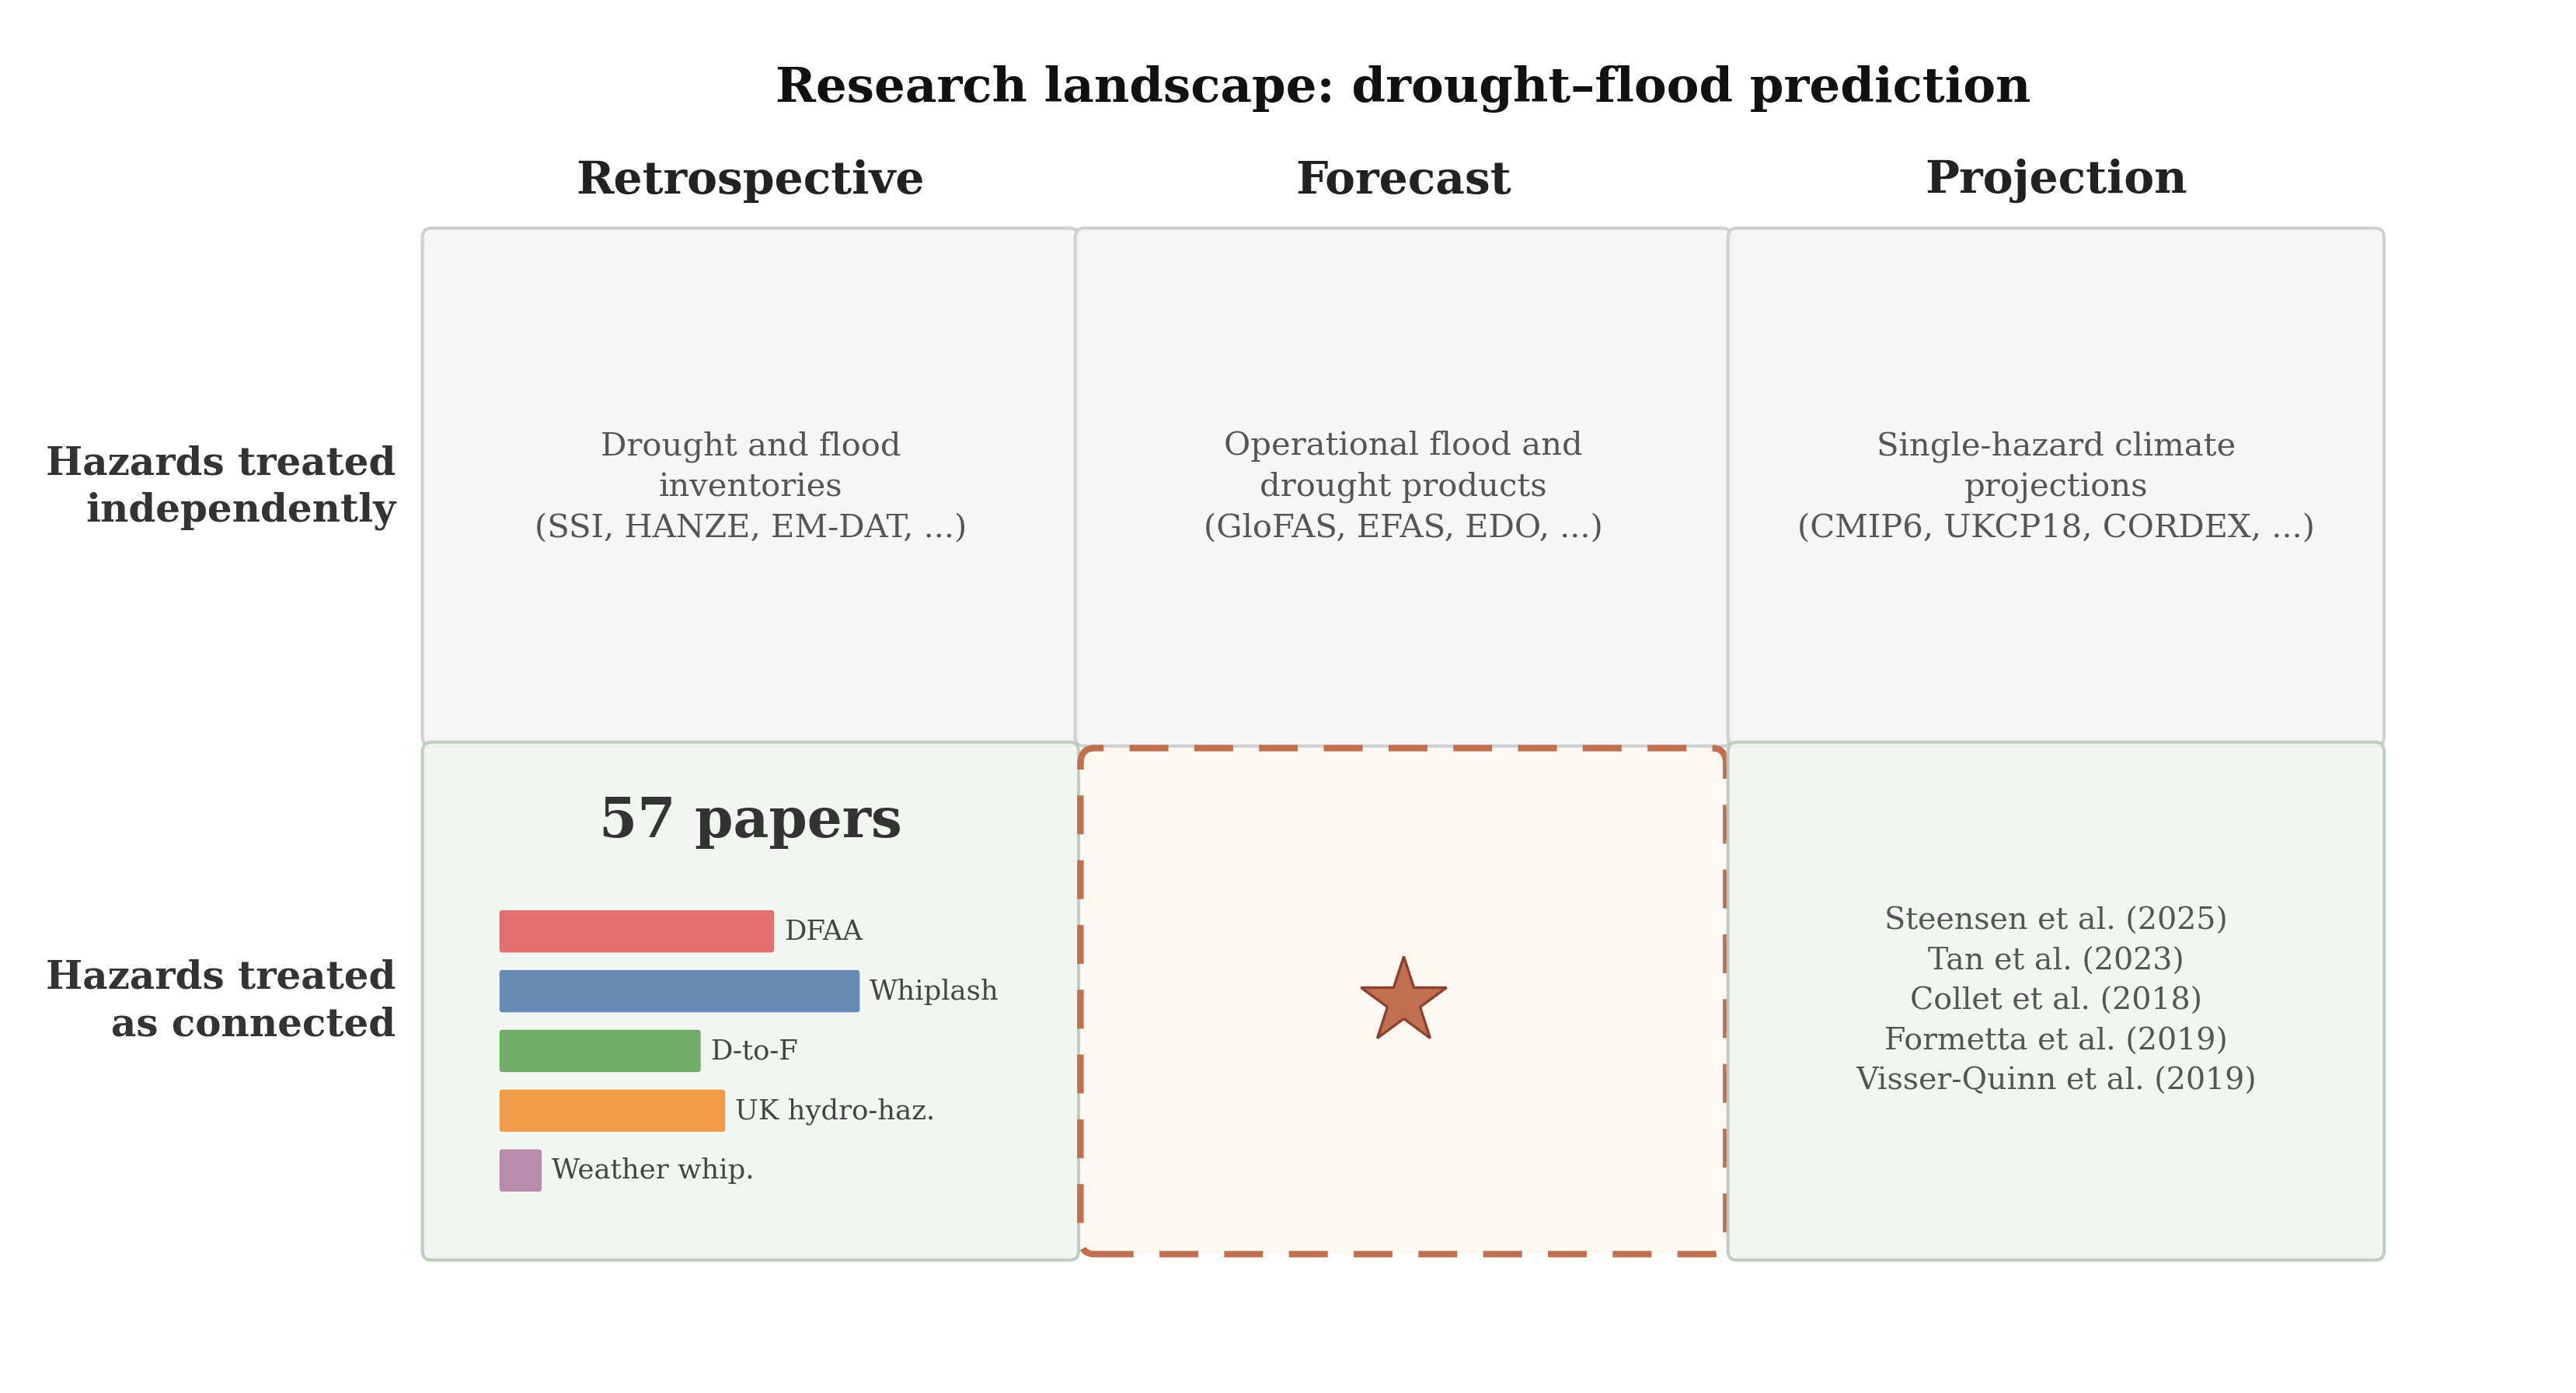
\includegraphics[width=0.88\textwidth, keepaspectratio]
        {research_landscape.png}

    \vspace{0.5em}
    {\footnotesize\color{gray!70}
     90 papers $\cdot$ 5 traditions \hspace{1em}
     {\color{statred}\ding{72}} = no forecast of connected drought--flood events}

\end{frame}

% --------------------------------------------------
% SLIDE 4: Could we forecast it?
% --------------------------------------------------
\begin{frame}{Is This Forecastable?}

    \centering
    \vspace{0.6em}

    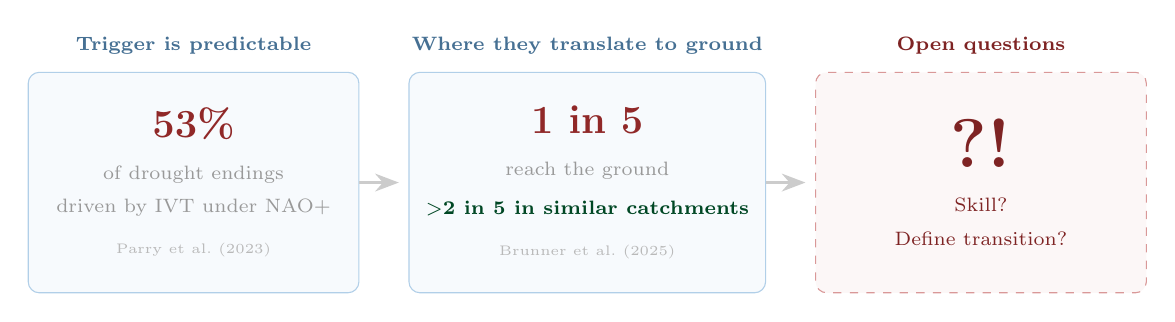
\begin{tikzpicture}[
        statbox/.style={minimum width=4.6cm, minimum height=2.8cm,
            align=center, rounded corners=4pt, inner sep=6pt},
        arr/.style={-{Stealth[length=3mm]}, very thick, gray!40}
    ]

    \node[statbox, draw=slideblue!50, fill=slideblue!5,
          minimum width=4.2cm] (b1) at (-5.0, 0) {
        {\Large\bfseries\color{statred!80!black} 53\%}\\[0.3em]
        {\scriptsize\color{gray!80} of drought endings}\\
        {\scriptsize\color{gray!80} driven by IVT under NAO+}\\[0.3em]
        {\tiny\color{gray!55} Parry et al.\ (2023)}
    };
    \node[font=\scriptsize\bfseries, text=slideblue!70!black,
          above=0.1cm of b1] {Trigger is predictable};

    \draw[arr] (b1.east) -- ++(0.5, 0);

    \node[statbox, draw=slideblue!50, fill=slideblue!5,
          minimum width=4.2cm] (b2) at (0, 0) {
        {\Large\bfseries\color{statred!80!black} 1 in 5}\\[0.3em]
        {\scriptsize\color{gray!80} reach the ground}\\[0.2em]
        {\scriptsize\bfseries\color{ucdgreen!70!black} {$>$}2 in 5 in similar catchments}\\[0.3em]
        {\tiny\color{gray!55} Brunner et al.\ (2025)}
    };
    \node[font=\scriptsize\bfseries, text=slideblue!70!black,
          above=0.1cm of b2] {Where they translate to ground};

    \draw[arr] (b2.east) -- ++(0.5, 0);

    \node[statbox, draw=statred!50, fill=statred!4,
          minimum width=4.2cm, dashed] (b3) at (5.0, 0) {
        {\Huge\bfseries\color{statred!70!black} ?!}\\[0.4em]
        {\scriptsize\color{statred!70!black} Skill?}\\
        {\scriptsize\color{statred!70!black} Define transition?}
    };
    \node[font=\scriptsize\bfseries, text=statred!70!black,
          above=0.1cm of b3] {Open questions};

    \end{tikzpicture}

\end{frame}

% --------------------------------------------------
% SLIDE 5: The approach (Pipeline)
% --------------------------------------------------
\begin{frame}{What's My Approach?}

    \centering
    \vspace{0.8em}

    \begin{tikzpicture}[
        pipebox/.style={
            minimum width=2.8cm, minimum height=2.4cm,
            align=center, rounded corners=5pt,
            inner sep=5pt, thick
        },
        arr/.style={-{Stealth[length=3mm]}, very thick, gray!40}
    ]

    % Pipeline boxes — getting noticeably darker left to right
    \node[pipebox, draw=slideblue!30, fill=slideblue!4,
          minimum width=2.2cm] (s1) at (-5.8, 0) {
        {\Large\color{slideblue!40!black} \faCloud}\\[0.4em]
        {\footnotesize\bfseries ECMWF}\\
        {\footnotesize\bfseries ensemble}
    };

    \draw[arr] (s1.east) -- ++(0.35, 0);
    \node[pipebox, draw=slideblue!45, fill=slideblue!10,
          minimum width=2.2cm] (s2) at (-3.0, 0) {
        {\Large\color{slideblue!55!black} \faTint}\\[0.4em]
        {\footnotesize\bfseries Hydro}\\
        {\footnotesize\bfseries model}
    };

    \draw[arr] (s2.east) -- ++(0.35, 0);
    \node[pipebox, draw=slideblue!60, fill=slideblue!18,
          minimum width=2.2cm] (s3) at (-0.2, 0) {
        {\Large\color{slideblue!70!black} \faChartLine}\\[0.4em]
        {\footnotesize\bfseries Standardised}\\
        {\footnotesize\bfseries index}
    };

    \draw[arr] (s3.east) -- ++(0.35, 0);
    \node[pipebox, draw=slideblue!75, fill=slideblue!25,
          minimum width=2.2cm] (s4) at (2.6, 0) {
        {\Large\color{slideblue!85!black} \faList}\\[0.4em]
        {\footnotesize\bfseries Track each}\\
        {\footnotesize\bfseries member}
    };

    \draw[arr] (s4.east) -- ++(0.35, 0);
    \node[pipebox, draw=statred!40, fill=statred!6,
          minimum width=2.6cm] (s5) at (5.5, 0) {
        {\Large\color{statred!60!black} \faRandom}\\[0.4em]
        {\footnotesize\bfseries Transition}\\
        {\footnotesize\bfseries probability}\\[0.2em]
        {\normalsize\bfseries\color{statred!80!black} 8/25 = 32\%}
    };

    % ML box — centred below
    \node[font=\small, text=gray!80, align=center,
          draw=gray!50, rounded corners=4pt, fill=gray!8,
          minimum height=0.9cm, minimum width=3.5cm] (ml) at (-1.6, -3.0)
        {\faRobot\hspace{0.4em} Machine learning?};

    % Arrow 1: ML left side to midpoint between box 1 and box 2 (post-process met)
    \coordinate (mid12) at ($(s1.east)!0.5!(s2.west)$);
    \draw[-{Stealth[length=2mm]}, thick, gray!45]
        (ml.west) to[out=170, in=-70, looseness=0.8] ($(mid12)+(0,-0.1)$);

    % Arrow 2: ML to hydro model box (replace/augment)
    \draw[-{Stealth[length=2mm]}, thick, gray!45]
        (ml.north) to[out=80, in=-80] ([yshift=-0.1cm]s2.south);

    \end{tikzpicture}

\end{frame}

% --------------------------------------------------
% SLIDE 6: Takeaways
% --------------------------------------------------
\begin{frame}{Takeaways}

    \begin{columns}[c, totalwidth=\textwidth]

        % Left: takeaways
        \begin{column}{0.68\textwidth}
            \vspace*{\fill}
            \centering
            \begin{tikzpicture}[
                iconcirc/.style={circle, minimum size=1.3cm, thick, align=center},
                lbl/.style={font=\normalsize, text=gray!15!black, anchor=west}
            ]

            \node[iconcirc, draw=statred!50, fill=statred!10] (i1) at (-3.5, 1.8)
                {\Large\color{statred!70!black}\faArrowUp};
            \node[lbl] at (-2.4, 1.8)
                {Transitions cause worse impacts};

            \node[iconcirc, draw=slideblue!60, fill=slideblue!12] (i2) at (-3.5, -0.2)
                {\Large\color{slideblue!70!black}\faSearch};
            \node[lbl] at (-2.4, -0.2)
                {Nobody has forecast them yet};

            \node[iconcirc, draw=ucdgreen!50, fill=ucdgreen!10] (i3) at (-3.5, -2.2)
                {\Large\color{ucdgreen!70!black}\faMapPin};
            \node[lbl] at (-2.4, -2.2)
                {Ireland as my testbed};

            \end{tikzpicture}
            \vspace*{\fill}
        \end{column}

        % Right: QR + contact
        \begin{column}{0.30\textwidth}
            \centering
            \vspace{1.2em}
            \begin{tikzpicture}
                % LinkedIn QR + icon
                \node[inner sep=0pt] (qrli) at (0, -1.0)
                    {
\includegraphics[width=2.2cm]{qrcode_linkedin.png}};
                \node[anchor=west, font=\large] at ([xshift=0.1cm, yshift=0.6cm]qrli.east)
                    {\color{slideblue!70!black}\faLinkedin};

                % Equal spacing: 0.8cm gap
                % Feedback QR + icon
                \node[inner sep=0pt] (qrfb) at (0, -3.5)
                    {
\includegraphics[width=2.2cm]{qrcode_feedback.png}};
                \node[anchor=west, font=\large] at ([xshift=0.1cm, yshift=0.6cm]qrfb.east)
                    {\color{gray!70}\faComment};

                % Name and email — same 0.8cm gap, centred on x=0
                \node[font=\footnotesize\bfseries, text=slideblue!80!black] at (0, -5.1)
                    {Lainey Ward};
                \node[font=\tiny, text=gray!40!black] at (0, -5.5)
                    {lainey.ward1@ucdconnect.ie};
            \end{tikzpicture}
        \end{column}

    \end{columns}

\end{frame}

% --------------------------------------------------
% SLIDE 7: References
% --------------------------------------------------
\begin{frame}{References}

    \vspace*{\fill}
    \centering

    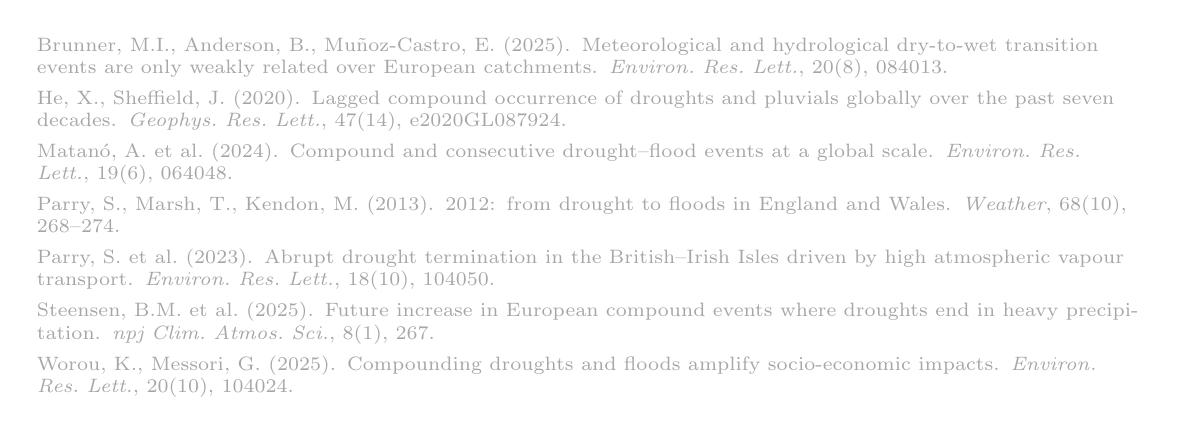
\begin{tikzpicture}
    \node[font=\scriptsize, text=gray!70, align=left, text width=14cm] at (0, 0) {
        Brunner, M.I., Anderson, B., Mu\~noz-Castro, E. (2025). Meteorological and hydrological dry-to-wet transition events are only weakly related over European catchments. \textit{Environ.\ Res.\ Lett.}, 20(8), 084013.\\[0.4em]
        He, X., Sheffield, J. (2020). Lagged compound occurrence of droughts and pluvials globally over the past seven decades. \textit{Geophys.\ Res.\ Lett.}, 47(14), e2020GL087924.\\[0.4em]
        Matan\'o, A. et al.\ (2024). Compound and consecutive drought--flood events at a global scale. \textit{Environ.\ Res.\ Lett.}, 19(6), 064048.\\[0.4em]
        Parry, S., Marsh, T., Kendon, M. (2013). 2012: from drought to floods in England and Wales. \textit{Weather}, 68(10), 268--274.\\[0.4em]
        Parry, S. et al.\ (2023). Abrupt drought termination in the British--Irish Isles driven by high atmospheric vapour transport. \textit{Environ.\ Res.\ Lett.}, 18(10), 104050.\\[0.4em]
        Steensen, B.M. et al.\ (2025). Future increase in European compound events where droughts end in heavy precipitation. \textit{npj Clim.\ Atmos.\ Sci.}, 8(1), 267.\\[0.4em]
        Worou, K., Messori, G. (2025). Compounding droughts and floods amplify socio-economic impacts. \textit{Environ.\ Res.\ Lett.}, 20(10), 104024.
    };
    \end{tikzpicture}

    \vspace*{\fill}

\end{frame}

\end{document}
